\section{Entwicklung zur DevOps-Kultur} \label{entwicklung}
Es ist denkbar, einen gewissen Teil von Continuous Delivery auch ohne DevOps einzuführen. Letztendlich bringen diese Ansätze weniger Vorteile mit sich. Hierfür muss es nicht zwingend fachlich organisierte Teams geben. Im Grunde reicht eine Kooperation der Abteilungen, um gemeinsam an der Continuous-Delivery-Pipeline zu arbeiten. Continuous Delivery verfolgt eine Vielzahl von Zielen. Einige können trotz reduzierter Pipeline erreicht werden. Hierfür ist keine umfangreiche Umorganisation notwendig.\\ Wenn Continuous Delivery vollständig umgesetzt werden soll, gelingt dies nur mit der Einführung von DevOps. Dies bedeutet eine fundamentale Änderung der Organisation. Eine solche Transformation ist mit einem erheblichen Aufwand verbunden und kann vor allem in großen Konzernen schwer umsetzbar sein. In diesem Kapitel wird darauf eingegangen, welche Aspekte zu berücksichtigen sind und welche Folgen diese Neuorientierung für Unternehmen hat [1].

\subsection{Umsetzung von Continuous Delivery}
Continuous Delivery ist lediglich eine technische Praktik, trotzdem hat diese Disziplin verschiedene Auswirkungen auf die Organisation. Continuous Delivery steht und fällt mit der Pipeline. Das Umsetzen einer einfachen Delivery-Pipeline kann mit simplen mitteln erfolgen. Vor allem zu Beginn eines Projekts kann der Aufbau einer solchen Pipeline verfolgt werden. Beispielsweise kann ein Unternehmen hier vorab mit den Phasen Commit und Deploy beginnen, da diese schließlich existieren müssen. Es ist dann möglich, die Pipeline im weiteren Verlauf schrittweise weiterzuentwickeln, indem entsprechende Phasen (z. B. automatisierte Tests) hinzugefügt werden. Wird Continuous Delivery zum Start eines Projekts eingeführt, kann dies auch bei der Auswahl der Technologien und Architekturen berücksichtigt werden [1]. \\ \\
Oft setzt Continuous Delivery an eine bestehende Codebasis an. Die bisherige Architektur ist gegebenenfalls nicht für den Einsatz von Continuous Delivery konzipiert worden. Wie eben erwähnt, müssen Prozesse zur Auslieferung der Software bereits bestehen, wodurch eine Delivery-Pipeline in gewisser Weise vorausgesetzt werden kann. Nur können diese Prozesse komplex sein. Das Ziel von Continuous Delivery ist allerdings, einen konstanten Fluss von Features und Codeänderungen durch die Pipeline zu erreichen. Hierbei muss der Value Stream betrachtet werden. Dies bezeichnet den derzeitigen Ablauf bis zum Release der Software. Werden die einzelnen Stationen betrachtet, lassen sich Optimierungsmaßnahmen ableiten. Es können beispielsweise Engpässe ermittelt werden, um den Fluss zu optimieren, auch wenn die Pipeline noch nicht gänzlich automatisiert ist. Dieses Verfahren wird als Value Stream Mapping bezeichnet und stellt eine wertvolle Analysetechnik dar, um bestehende Pipelines schrittweise zu verbessern. Obwohl Continuous Delivery eine Sammlung verschiedener Werkzeuge ist, reicht es bei der Umsetzung nicht, schlicht entsprechende Techniken und Tools zu verwenden. Solange die Prozesse innerhalb der Organisation nicht einwandfrei ablaufen, kann hier keine signifikante Steigerung der Effizienz erreicht werden [5]. Der Schlüssel hierfür ist DevOps, da das Know-How aus ausschlaggebenden Abteilungen zusammenkommt [1].

\subsection{Umsetzung von DevOps}
Viele Unternehmen sind bereits dabei, DevOps erfolgreich umzusetzen. Allerdings bleiben nach wie vor kritische Barrieren bei der Entwicklung, wie sie im folgenden Kapitel näher beschrieben werden. Dabei ist die größte Hürde die Angst vor Veränderungen (siehe vorherige Abneigung gegenüber Clouds) [3]. Um diese Philosophie anzuwenden gibt es verschiedene Möglichkeiten, allerdings muss klar sein, was DevOps für das Unternehmen bedeutet. Zwei der größten Hindernisse, diese Disziplin erfolgreich umzusetzen, sind die Unternehmensarchitektur sowie Unternehmenskultur, die davon beeinflusst werden.

\subsubsection{Kultur}
Die Unternehmenskultur ist von der Transformation betroffen. Es ist wichtig, eine Kultur zu schaffen, in welcher alle Menschen der Organisation bei der Verfolgung gemeinsamer Ziele zusammenarbeiten. Bei DevOps wird stets die primäre Bedeutung der Kultur hervorgehoben. Der Fokus liegt auf einer effektiven Zusammenarbeit der Entwickler und IT-Betriebsteams. Durch diese Kollaboration, welche die Unabhängigkeit und Selbständigkeit der Teams fördert, bedarf es einer zentralen Kontrolle nur noch um bestimmte Rahmenbedingungen zu etablieren und zu kontrollieren.\\ \\    
Ein Extrembeispiel bezüglich der im Unternehmen verfolgter Kultur ist wohl Netflix mit seiner Simian Army. Dabei werden beispielsweise regelmäßig zufällige Instanzen ihrer Architektur zerstört, um (kontrollierte) Unfälle zu simulieren. Somit wird das unabhängige Funktionieren der Komponenten sichergestellt. Leistungsstarke Unternehmen warten also nicht darauf, dass Ausfälle passieren, um daraus zu lernen und sich zu verbessern. Durch dieses radikale Vorgehen bzw. diese Architektur des Systems lassen sich Optimierungen ableiten [3].

\subsubsection{Architektur}
Continuous Delivery sowie DevOps und die somit weitgehend autonome Teams bedeuten auch für die Architektur der Lösungen eine Herausforderung. Zum einen erfordert es ein gewisses Maß an Abstimmung zwischen den Teams, um gemeinsam die Architektur des Systems zu entwickeln. Das Festlegen der Architektonik durch eine zentrale Instanz stellt einen Widerspruch zu den eigenverantwortlichen Teams dar. Die Abstimmung erfolgt über entsprechend definierte und moderierte Meetings, an denen auch zentrale Architekten teilnehmen können. Zum anderen muss die Delivery-Pipeline des Systems entsprechend aufgebaut bzw. angepasst werden.\\ Wird an einer Stelle des Systems eine Änderung durchgeführt, muss nicht die ganze Pipeline durchlaufen werden. Das würde zum Testen des gesamten Systems führen. Zwar kann dies durchaus sinnvoll sein, da Fehler in einer Komponente erst durch ein Fehlverhalten einer anderen Komponente auftreten können (Seiteneffekte), trotzdem wäre die Folge ein unnötig großer Aufwand und ein verzögertes Feedback. Durch Continuous Delivery ergibt sich demnach eine andere technische Umsetzung der Komponenten, denn jede Komponente sollte als eigene Einheit betrachtet und implementiert werden. Somit lassen diese sich unabhängig voneinander als Teil des Gesamtsystems deployen und durchlaufen jeweils eine eigene Pipeline. Das schnelle Feedback und die angestrebte Risikominimierung wird hierdurch erreicht. Schleicht sich ein Fehler ein, kann er leichter identifiziert werden, da die Deployment-Einheiten wesentlich kleiner sind. Auch die Kommunikation zwischen den Komponenten ist betroffen. Wird jede Komponente als eigenständiger Service als Teil eines verteilten Systems implementiert, muss die Kommunikation angepasst werden. Potenzielle Lösungen bieten REST oder entsprechende Message Oriented Middleware. Möglichst kleine, lose gekoppelte und gekapselte Module sind somit für Continuous Delivery sinnvoll (im Rahmen der objektorientierten Programmierung werden hier die Prinzipien des SOLID-Designs verfolgt). Die daraus resultierenden verteilten Systeme machen das Design entsprechender Schnittstellen zu einem wichtigen Faktor [1]. \\ \\
Durch verschiedene Anpassungen der Architektur und den bisher erwähnten Anforderungen an die Organisation ergibt sich ein umfangreiches Zusammenwirken von Continuous Delivery und dem Softwarearchitekturansatz von Microservices. Microservices genügen den Anforderungen an einer Architektur für ein Continuous Delivery-System und setzen auch andere Aspekte (Technologiefreiheit, unabhängige Einheiten etc.) um [1]. Diese architektonischen Eigenschaften wurden hier sogar explizit priorisiert [3]. Somit ist die Einführung von Continuous Delivery im Grunde eine Einführung von Microservices. Bei der Umsetzung von Continuous Delivery muss die Architektur der Software angepasst werden. Lediglich die Prozesse anzupassen bzw. zu ändern, ist nicht ausreichend [1].

\subsubsection{Technolgie}
Wie erwähnt, ist die Technologiefreiheit ein Aspekt dieses Ansatzes. Da die Teams weitgehend autonom handeln können, übernehmen sie die vollständige Zuständigkeit bei der Auswahl ihrer Implementierungstechnologien. Frameworks, Programmiersprachen oder Application Server werden eigenverantwortlich ausgewählt. Diese Entscheidungen haben an einigen Stellen Einfluss auf die Pipeline. Programmiersprachen beeinflussen beispielsweise die Geschwindigkeit der Compiler, wodurch die benötigte Zeit beim Durchlaufen der Pipeline beeinflusst wird. Technologieentscheidungen haben demnach einen direkten Einfluss auf die Continuous-Delivery-Pipeline [1].\\ \\
Treten mit den ausgewählten Technologien Probleme auf, muss sich auch nur dieses Team mit der Behebung auseinandersetzen. So lässt sich eine Vielzahl von Technologien im Unternehmen nutzen, während eine klassische Organisation diese möglichst einschränken und kontrollieren möchte. So sollen beispielsweise potentielle Risiken beim Interagieren der Komponenten minimiert werden. Teilen sich Komponente und Projekte dieselbe Programmiersprache und Infrastruktur, kann jeder Entwickler mit der entsprechenden Technologie umgehen. Es kann jedes Projekt in gewisser Weise unterstützt werden. Auch der Betrieb kann sich so auf eine Technologie fokussieren und ist mit möglichen Problemen dieses Technologie-Stacks vertraut. Bei DevOps hingegen steht die Freiheit, eigene Entscheidungen zu treffen im Vordergrund. Ein Standard-Stack kann etabliert werden, indem auf Erfahrungen anderer Teams zurückgegriffen wird. Somit könnte es bereits eine Ansammlung von Tools geben, welche für andere Teams nutzbar ist [1]. 

%\begin{figure}[h!]
%	\centering
%	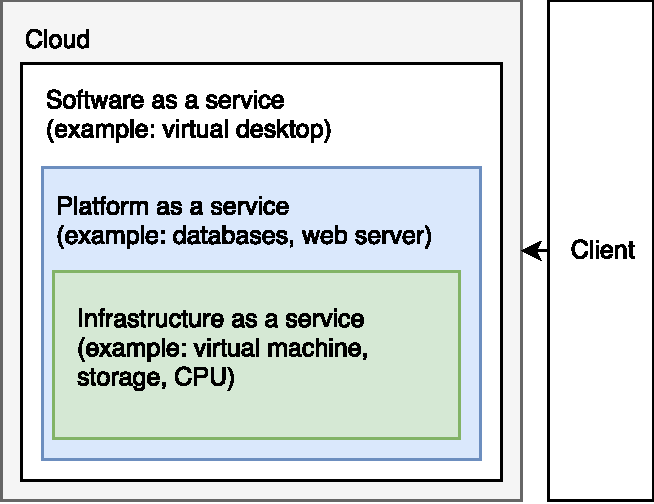
\includegraphics[width=0.8\linewidth]{images/servicemodules.pdf}
%	\caption{Cloud-Servicemodelle} %Generelle
%	\label{fig:cnn_structure}
%\end{figure}